\section{Overview of Auto311}

Auto311 is developed to autonomously handle non-emergency calls by engaging in interactive conversations with callers. An outline of our system's structure is shown in Figure \ref{fig:sys_overview}. The system comprises five key components: the \textit{conversational interface} for interacting with callers, the \textit{handover control} to transfer calls to human operators if needed, the \textit{incident type prediction} module to identify probable incident types, the \textit{information itemization} module to organize details in case reports, and the \textit{confidence-guided report generation and dialogue optimization} module for generating informed reports and optimizing subsequent conversations using confidence guidance.

% Auto311 has been designed to autonomously manage non-emergency calls, engaging in interactive conversations with non-emergency callers. An overview of our system's architecture is presented in Figure \ref{fig:sys_overview}. The system consists of five integral components: the \textit{conversational interface}, which facilitates interaction with callers; the \textit{handover control} function, responsible for directing calls to human operators when urgent situations arise; the \textit{incident type prediction} module, which identifies the most probable incident type(s) associated with the ongoing call; the \textit{information itemization} module, responsible for categorizing information into appropriate sections within the case report; and the \textit{confidence-guided report generation and dialogue optimization} module, ensuring the generation of a well-informed report and the optimization of subsequent dialogues with obtained confidence guidance.


% Auto311 is designed to handle non-emergency calls automatically. It interacts with the non-emergency callers in back-and-forth conversations. An overview of our system is shown in Figure \ref{fig:sys_overview}. There are five components of our system, including a \textit{conversational interface} to interact with the caller, a \textit{handover control} function to reroute calls to real operators in case of urgencies, an \textit{incident type prediction} module to indicate the most likely incident type(s) of the ongoing call, an \textit{information itemization} module to itemize the information based on the blank fields in the case report, and a \textit{confidence-guided report optimization} to ensure the report is generated. Future dialogue is optimized with obtained module outputs and corresponding confidence scores.

\begin{figure}[h]
    \centering
    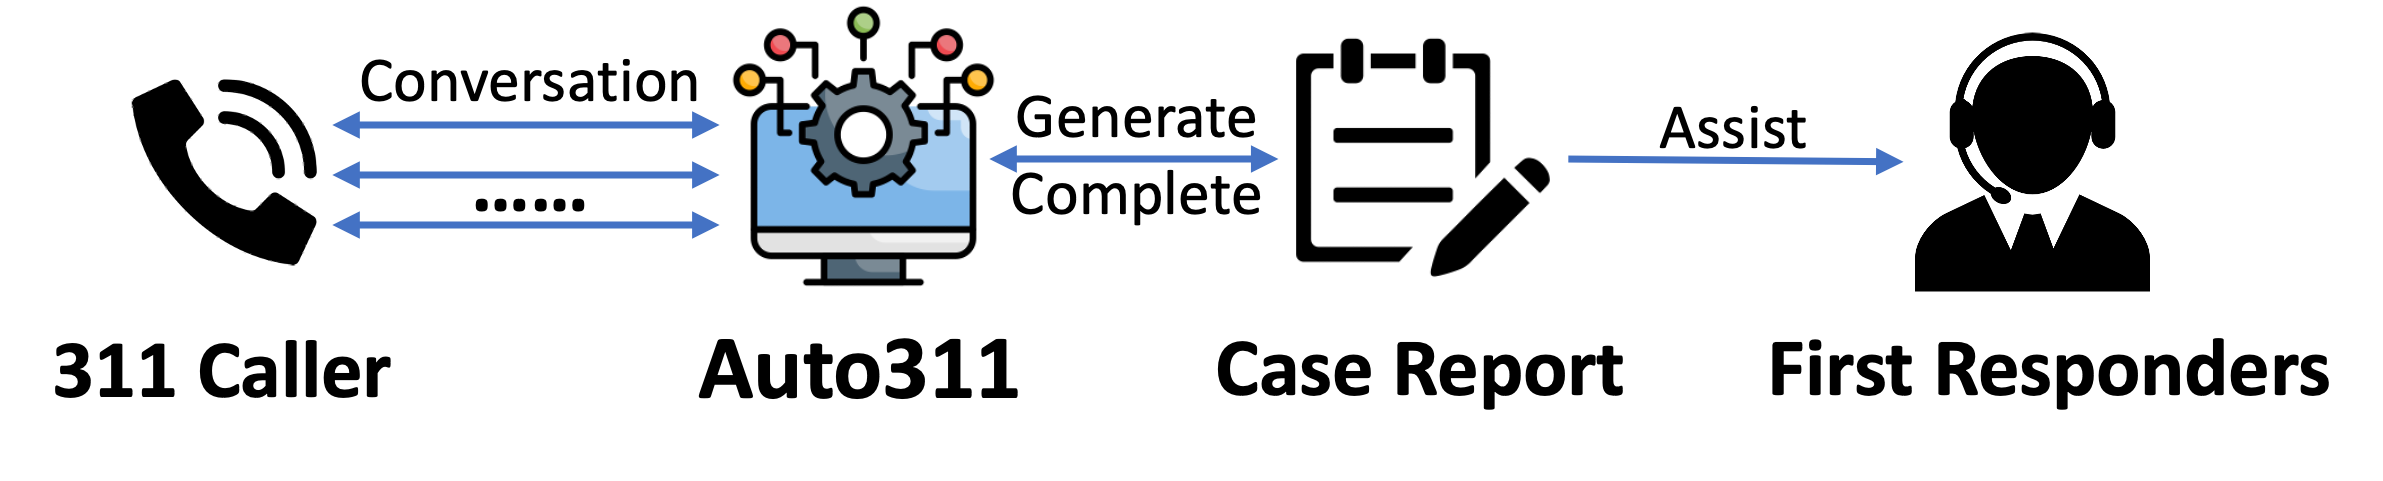
\includegraphics[width=0.4\textwidth]{figures/system_overview.png}
    \caption{Auto311 in Emergency Response}
    \label{fig:sys_overview}
    \vspace{-0.5cm}
\end{figure}

During runtime, as shown in Figure \ref{fig:sys_logic}, when a caller initiates contact, the \textit{conversational interface} starts the dialogue with opening questions, collecting essential information like the caller's name and incident location. Each response from the caller forms an utterance. Subsequently, the \textit{handover control} function evaluates whether human operator intervention is required for the call. The call proceeds to subsequent modules only if the handover is not needed. At the same time, the \textit{incident type prediction} module forecasts the most likely incident type(s) for report generation, while the \textit{information itemization} module provides potential details from the caller's utterance to fill the report's sections. Additionally, the \textit{confidence-guided report generation and dialogue optimization} module constantly monitors confidence scores to ensure the report is filled with high confidence, thereby optimizing follow-up conversations.

% During runtime, as illustrated in Figure \ref{fig:sys_logic}, when a caller initiates contact, the \textit{conversational interface} commences the dialogue by presenting opening questions, gathering fundamental information such as the caller's name and incident location. With each turn, the caller's response is captured as an utterance. Once the utterance is obtained, the \textit{handover control} function assesses whether a human operator's intervention is necessary for the ongoing call. Only if the handover control function's criteria are met does the call progress to subsequent modules. Concurrently, the \textit{incident type prediction} module anticipates the most probable incident type(s) to facilitate report generation, while the \textit{information itemization} module supplies potential details from the caller's utterance to complete the report's blank sections. Moreover, the \textit{confidence-guided report generation and dialogue optimization} module continuously monitors confidence scores to ensure that the report is enriched with maximum confidence, thereby optimizing follow-up dialogues.

% At runtime, shown in Figure \ref{fig:sys_logic}, upon a caller dials in, the \textit{conversational interface} initializes the dialogue with opening questions, querying basic questions, such as the caller's name and the location of the incident. At every turn, the caller's response is collected as an utterance. After obtaining the utterance, the \textit{handover control} function decides if a human operator needs to interfere with the current call. Only when the call clears the concerns of the handover control function, will it be passed to the subsequent modules. Meanwhile, the \textit{incident type prediction} module predicts the most likely incident type(s) to guide the report creation, and the \textit{information itemization} module offers potential information from caller utterance to the blank fields in the report. The \textit{confidence-guided report generation and dialogue optimization} module further tracks the confidence scores to make sure the report is updated with the maximized confidence so that the follow-up dialogues are optimized. 

\begin{figure*}[t]
    \centering
    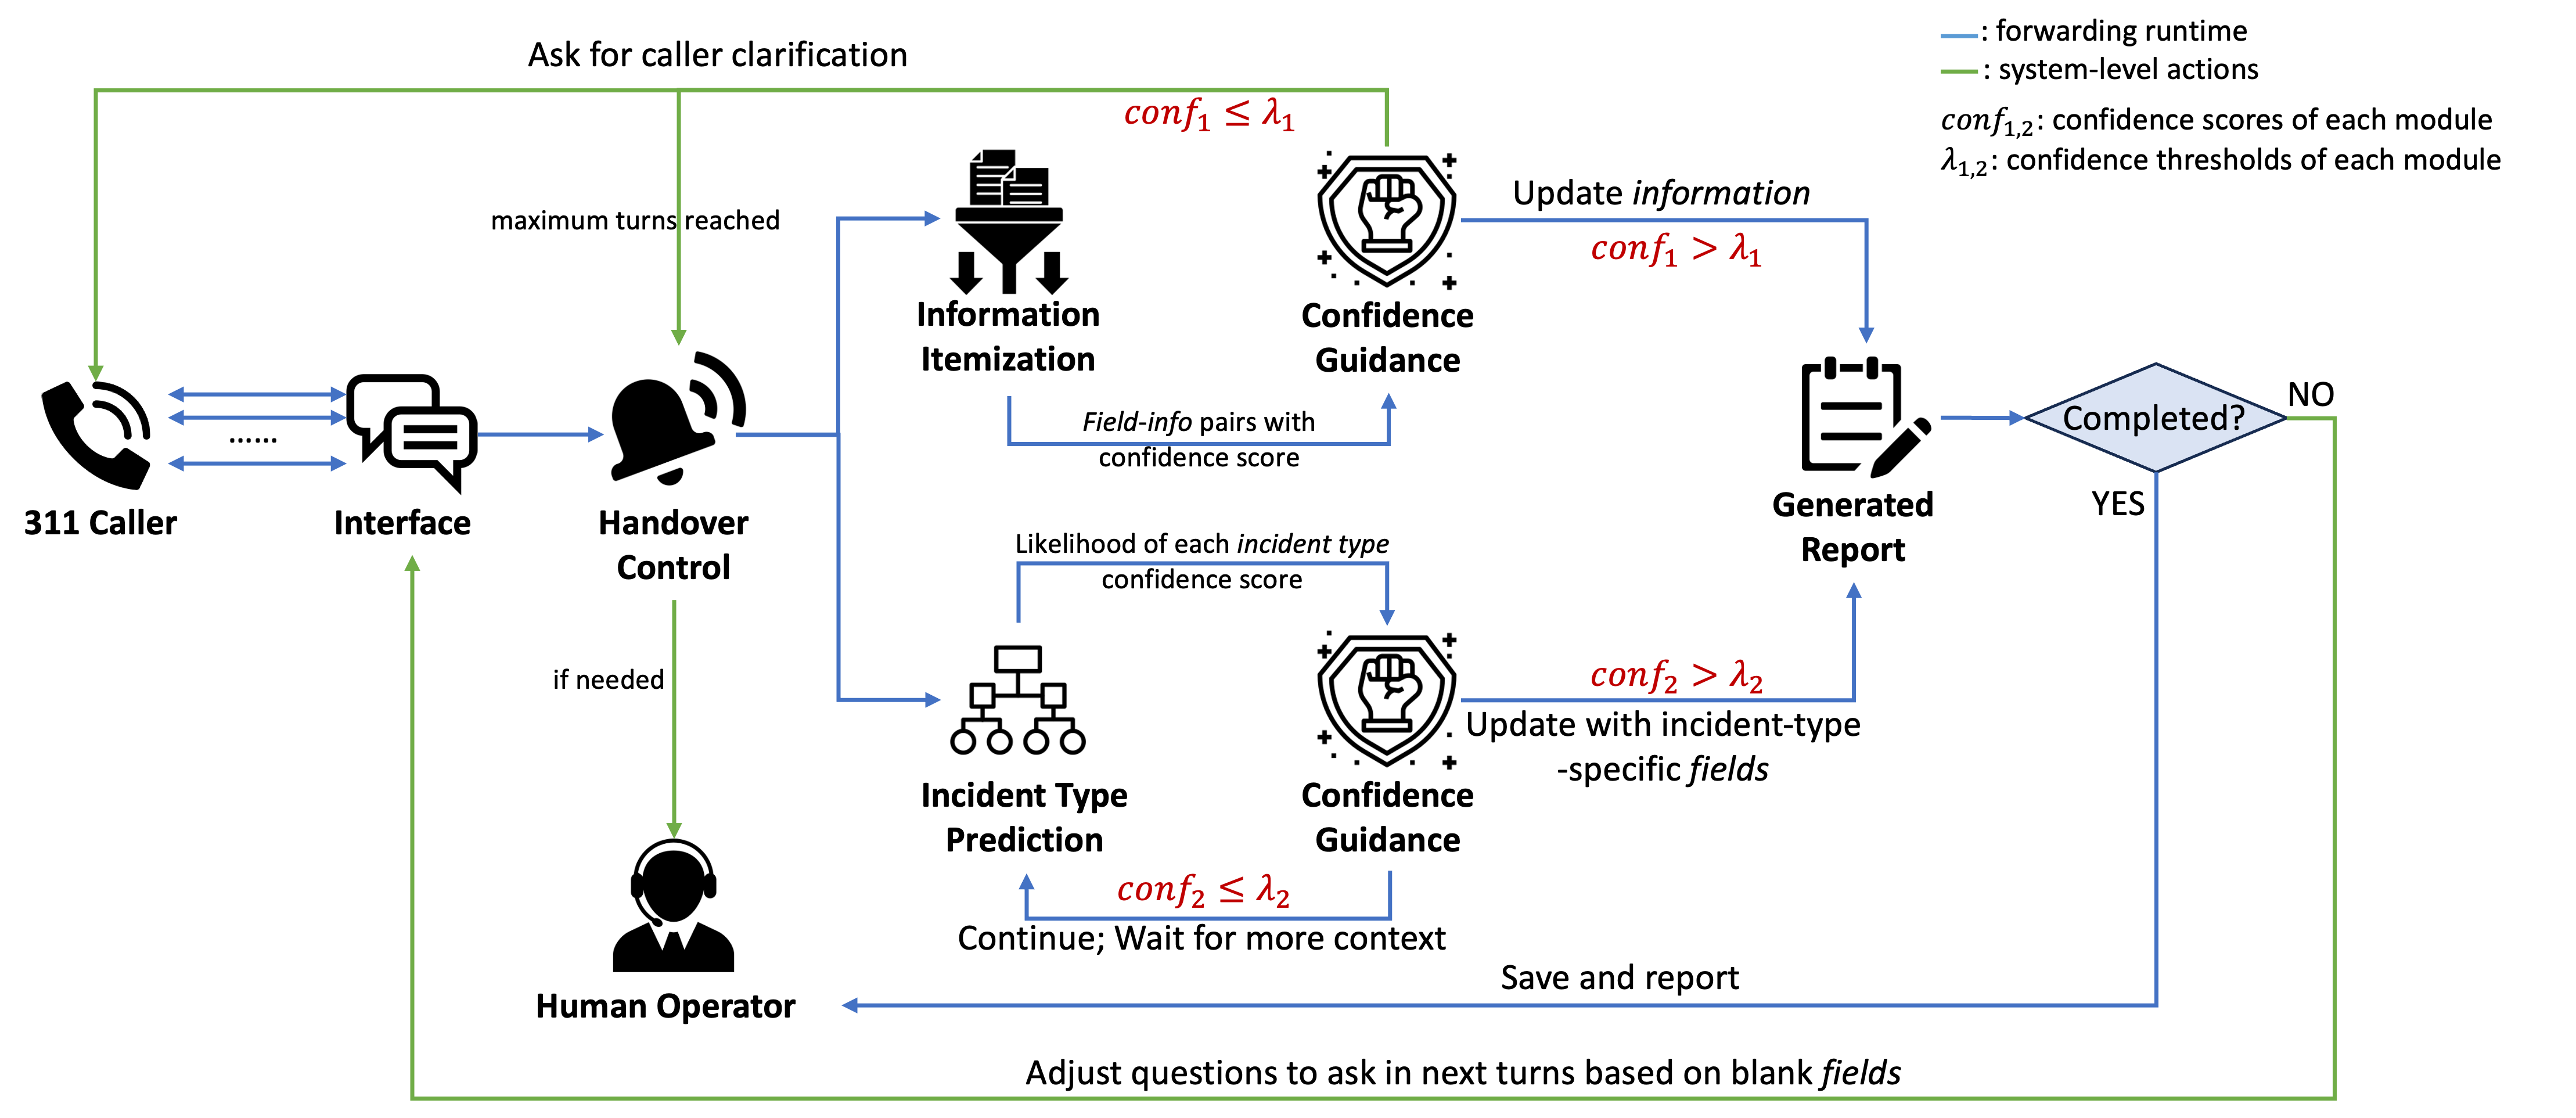
\includegraphics[width=0.9\textwidth]{figures/system_logic.png}
    \caption{Confidence-guided System Design}
    \label{fig:sys_logic}
    \vspace{-0.5cm}
\end{figure*}

% \subsubsection{Case Report vs Question List}
Importantly, the case report referred to here differs from the question list within the conversational interface. The question list stores upcoming inquiries for the interface, while the case report shapes the subsequent dialogue by updating the question list with its incomplete sections after each conversation turn.

% It is worth noting that the case report mentioned here is different from the question list in the conversational interface. The question list stores the next questions to ask for the conversational interface. However, the case report organizes the follow-up dialogue by updating the question list with its uncompleted fields after each conversation turn.

% in the following aspects: (1) the question list contains questions to ask in the next turns in the conversation, however, the case report consists of blank fields that need to be completed by the information itemization module; (2) the question list can be extended with blank fields with missing or low-confident answers while the case report can be extended by more specific fields under the predicted incident type from the incident type prediction module.

\subsection{Conversational Interface}

The conversational interface supports both voice and text inputs. Employing state-of-the-art audio transcription tools, notably the OpenAI Whisper model \cite{openai_whisper_2022}, this interface adeptly transforms speech into text, accommodating a range of accents. For text-to-speech functionality, we harness advanced audio generation tools like the Suno-AI Bark model \cite{bark}, acclaimed for producing realistic voices within a lightweight model framework. Beyond speech-to-text and text-to-speech conversion, the interface engages in conversations using a dynamically updated question list. This list determines the query sequence and guides the interface's speech-to-text conversion process.


% The conversational interface accommodates both voice and text formats. Leveraging cutting-edge audio transcription tools, specifically the OpenAI Whisper model \cite{openai_whisper_2022}, this interface proficiently converts speech to text while being adept at handling diverse accents. For text-to-speech generation, we rely on advanced audio generation tools such as the Suno-AI Bark model \cite{bark}, renowned for its capacity to produce remarkably realistic voices while maintaining a lightweight model size. Beyond the realm of text-to-speech and speech-to-text conversion, the conversational interface engages in interactions using a dynamically updated question list. This list dictates the sequence of questions to pose and serves as a guide for the interface's speech-to-text conversion process.

% The conversational interface supports both voice and text formats. Powered by one of the state-of-the-art audio transcription tools, the OpenAI Whisper model \cite{openai_whisper_2022}, the conversational interface is capable of speech-to-text transcription with robustness to different accents. Regarding backward text-to-speech generation, we also employ state-of-the-art audio generation tools, like the Suno-AI Bark model \cite{bark}, which guarantees highly realistic voice generation and light-weighted model size. Besides text-to-speech and speech-to-text generation, the conversational interface carries out the interactions with a question list that is dynamically updated each turn. The question list contains the next questions to ask and guides the speech-to-text generation of the interface. 

% In our settings, at the beginning stage, our interface initializes the conversation with the same opening question from a real operator: ``What is the location of the emergency?''. The starting question list only contains the following 4 questions: (1) what is the location of the emergency? (2) what is your name? (3) what is your best contact number? (4) Tell me what is going on. Then, the follow-up question list is generated at runtime based on the outputs from the next modules.

\subsection{Always-on Handover Control}

% The handover control module is kept active anytime during the runtime in case the current call needs to be rerouted to human operators. During our collaboration with the local call center, we further specify the following cases that trigger our handover control module: (1) when downstream modules return with exceptions, e.g., uncertain information; (2) when the caller keeps requesting to interact with a human operator, e.g., the caller says ``real operator'' or ``real human'' in the latest utterance; (3) early alerting for any potential urgency. The first case is handled inside system actions. For example, when Auto311 is uncertain about the itemized information, it asks the caller for clarification. We set the maximum turns of clarification to 3. Once the maximum is reached, we consider Auto311 faces exceptions and the handover control is triggered. To deal with the rest two cases, we develop an intuitive rule-based detection with high vigilance for future interpretability and control for the local call center team. We utilize Latent Dirichlet Allocation (LDA) \cite{blei2003latent} to produce a sensitive word list after manual review. We combine both nature language processing (NLP) features \cite{nltk} like stem, lemma, part-of-speech tags, and shallow parsing tags along with hand-coded patterns to figure out independent rules to trigger the handover control, ceasing system interaction. Please refer to the appendix for more details. Meanwhile, the patterns and sensitive words are not exhaustive; future usage expands the trigger conditions. However, this process goes beyond the scope of the current paper.

The handover control module remains active throughout runtime, redirecting calls to human operators when necessary. Collaborating with DEC, we identify specific scenarios that activate this module: (1) downstream module exceptions, like uncertain information; (2) caller's repeated request for human interaction; (3) proactive alerts for potential urgency. The first case is managed within system actions. For example, when Auto311 seeks clarification due to uncertain details, it limits such queries to three turns. Exceeding this threshold triggers exceptions and activates handover control. Addressing the other two cases, we develop an interpretable rule-based detection mechanism, prioritizing interpretability and control. Using Latent Dirichlet Allocation (LDA) \cite{blei2003latent}, we curate a sensitive word list through manual review. Our approach combines natural language processing (NLP) features \cite{nltk}, such as stemming, lemmatization, part-of-speech tags, and shallow parsing, with custom patterns to establish rules activating handover control, thus ending system interaction. More details are available in the appendix. Note that patterns and sensitive words are not exhaustive, allowing future expansion of trigger conditions. However, the broader process is beyond this paper's scope.

% The handover control module remains active throughout runtime to reroute calls to human operators as needed. Collaboration with the local call center leads us to identify specific scenarios that activate this module: (1) when downstream modules encounter exceptions, such as uncertain information; (2) when the caller repeatedly expresses a desire to communicate with a human operator; (3) proactive alerting for potential urgency. The first case is managed within system actions. For instance, when Auto311 is uncertain about detailed information, it seeks clarification from the caller, limiting such queries to three turns. If this threshold is reached, Auto311 deems exceptions present and triggers the handover control. To address the other two cases, we've developed an easily interpretable rule-based detection mechanism with a strong focus on future interpretability and  control. Employing Latent Dirichlet Allocation (LDA) \cite{blei2003latent}, we curate a sensitive word list via manual review. Our approach combines natural language processing (NLP) features \cite{nltk}, such as stemming, lemmatization, part-of-speech tags, and shallow parsing, with custom-coded patterns to establish distinct rules that activate the handover control, thus discontinuing system interaction. Further details are available in the appendix. It's important to note that the patterns and sensitive words are not exhaustive, leaving room for the expansion of trigger conditions in future applications. However, this broader process falls outside the scope of this paper.

\subsection{Incident Type Prediction}
\label{subsec:prediction}

The incident type prediction module utilizes contextual information from previous caller utterances. The module takes the overall context covering all prior utterances as input. Since a context can involve multiple incident types, we apply a multi-layer hierarchical structure and bootstrap-like procedure for classification. This tracks the possibility of the call belonging to each incident type (see Confidence-guided System Design for details). The hierarchical structure and iterative procedure enable the prediction module to handle multiple incident types per call using full conversational context.

% The contextual information from previous utterances facilitates the incident type prediction module. The module input is the overall context covering all previous caller utterances. Considering it is possible for a context to involve more than more incident types, we apply a multi-layer hierarchy structure and a bootstrap-like procedure for this classification to keep track of the possibility of the call belonging to each incident type, refer to more details in Section Methodology.

\subsection{Information Itemization}
\label{subsec:itemization}

The information itemization module completes empty case report sections by quoting the caller's utterances. This involves narrative fields seeking explanatory details and yes/no fields confirming facts. For narratives, we leverage extractive question-answering frameworks - the blank fields are inputs, and outputs quote relevant caller utterances. Yes/no fields become binary classification, predicting yes or no from the last utterance. Unlike incident prediction using all contexts, itemization considers only the latest utterance. 

% The information itemization module has a specific goal: to complete the empty sections in a case report quoting information from what the caller says. This involves two main types of fields: one that asks for a narrative explanation, such as where the incident happened, and another that seeks a simple ``yes'' or ``no'' based on what the caller says, like ``Are you the property owner?''. To deal with the first type, leveraging the ability of existing extractive question-answering frameworks, this module takes the blank fields in the case report as input and outputs the most relevant information by quoting the caller utterance segments. Meanwhile, we formulate the second type as a binary classification task. Different from the incident type prediction, which considers all previous contexts, this information itemization module considers only the last caller utterance as context. 

% Before the model is trained, we thoroughly examine our dataset and the local call center's guidelines for various incident types. We annotate the audio transcriptions to form our dataset in field-information pairs, which enables the training of this module. Different from the incident type prediction, which considers all previous contexts, this information itemization module considers only the last caller utterance as context. 

\subsection{Confidence-guided Report Generation and Dialogue Optimization}

This module updates the report and optimizes dialogues as the conversation progresses. See technical details in Section Confidence-guided System Design.

% The iterative report optimization and dialogue assistance allow dynamically improving reports as the conversation progresses.

% This module targets the optimization of the generated case report during every turn of the ongoing conversation and further assists dialogue organization. We discuss more technical details in Section Confidence-guided System Design.


% Our system assists dispatchers by suggesting likely incident types and itemizing key information to answer essential case report questions. The system, depicted in Fig. \ref{fig:sys_overview}, comprises incident type prediction and information itemization modules. It does not participate directly in dispatcher-caller conversations; rather, it generates an evolving answer sheet for dispatcher review and revision during the interaction. Fig. \ref{fig:running_example} demonstrates module cooperation within a single conversation turn, showcasing assistance for dispatchers.

% % Our system is designed to assist the dispatchers by (1) suggesting the most likely incident type of the ongoing call and (2) highlighting key information that would potentially answer the essential questions to file an internal case report. Thus, besides the handover control, there are two main modules in our system, see Fig.\ref{fig:sys_overview}: call dispatching and information extracting. Our system does not directly participate in the conversation between the dispatcher and the caller, it aims to generate an answer sheet for the dispatcher every turn as the conversation goes on, and the dispatcher has full access to review and revise the answer sheet anytime during the conversation. To better demonstrate how these two modules help with the dispatcher and interact with each other, we provide a running example, see Fig.\ref{fig:running_example} within one single turn of the conversation.

% Given previous findings on potential urgent situations underlying calls, we develop a \textbf{handover control} that interrupts system interference and routes the call to the dispatcher when more urgent incidents are detected, acknowledging each call's severity.

% % Based on the findings in the previous section, we acknowledge the potentially life-threatening situation behind each call, We develop a \textbf{handover control} in case the ongoing call is identified as an emergency call instead. The handover control interrupts the interference from our system and leaves the dispatcher the only participant during the call once there is any sign of an emergency is detected.

% \subsection{Call Dispatching Module}

% We track user utterances, maintaining overall context information passed to the call dispatching module. This multi-class classification module outputs the likelihood of categorizing the call into each incident type. The final prediction assists rather than replaces the dispatcher's decision-making, with the dispatcher retaining full control to alter outputs. The most likely incident-type queries associated with follow-up questions from the DEC question card, e.g., ``What is the vehicle color?'' for abandoned vehicles. These questions are appended to the information extracting module's question list.

% % During the call, we track every user utterance and maintain overall context information. The context information is passed to the call dispatching module. We model the whole process as a multi-class \textbf{classification} task and train the module to output the likelihood of whether the current call should be categorized into each incident type. The final prediction is provided to the dispatcher in a soft way, which means it only aims to assist the decision maker (dispatcher) instead of being the decision maker. Meanwhile, the dispatcher has full control over the module and can change the output anytime during runtime. After having the most likely incident type, this module queries all the follow-up questions from the DEC's question card specifically under that incident type, e.g., ``what is the color of the vehicle?'' under the abandoned vehicle category. Those follow-up questions are passed and appended to the question list in the information extracting module.

% \subsection{Information Extracting Module}

% The information extracting module focuses on extracting key information from the latest utterance to fulfill the essential questionnaire for internal reports. We model this as a QA pipeline trained to mark start and end indices in an utterance to answer a given question. The question list contains essential questions, starting with common questions before incident types are confirmed. Once confirmed, incident-specific questions are added, enabling the handling of additional caller-volunteered information. If there is only one single possible incident type confirmed, we will only query that certain incident type and follow DEC's question card, which contains all procedural questions that need to be further answered to complete the report. If there are multiple incident types detected, the question list will be updated using all relevant questions belonging to the detected incident types. Our confidence-checking functions make sure only the incident type(s) and its corresponding question-answer pairs with high internal consistency will be reported to the dispatcher.

% % The information extracting module mainly focuses on the latest user utterance and attempts to extract the key information from the latest utterance to fulfill the questionnaire that is essential to complete an internal report. We model the process as a \textbf{Q\&A-like pipeline}. This module is trained to mark the start and end indices in a given utterance to answer a given question. Meanwhile, the question is not limited to the proposed question by the dispatcher. Based on the findings from the previous section, there is a chance that the caller could convey additional information during the conversation, thus, we set up a question list for essential questions to ask. At initial turns, or before an incident type is confirmed, the question list only consists of common questions, which are not specific to any of the incident types. Once the incident type is confirmed, the question list will be extended with more incident-specific questions.

% \subsection{Confidence Checking Function}
% Confidence checking participates in both key modules, providing predictions and confidence scores indicating certainty. Low confidence suggests dispatchers carefully consider adopting predictions. We develop rules during runtime to strategically utilize the confidence scores. At the system level, the implementation of several procedural rules allows our system to make confidence-aware choices aimed at maximizing overall confidence scores throughout the conversation. In Fig. \ref{fig:dryrun}, further explanation elucidates confidence checking's system influence. Initially, system interactions initialize with the human operator's opening question: ``What is your emergency location?''. Concurrently, the question list commences with this location query alongside other questions commonly imperative for most incident types. Post-questioning, the system awaits and analyzes caller utterances for contextual information. Leveraging context, both modules generate predictions and associated confidence scores. Parallel module-specific methods determine prediction-confidence adoption. For information extraction, firm adoption only occurs for question-answer pairs exceeding the confidence threshold; clarification requests elicit below-threshold pairs until exceeding the threshold. Similarly, the call dispatching module only accepts the incident type and then updates the question list using retrieved incident-specific questions given sufficient confidence. However, immediate clarification does not occur. Instead, the system remains silent until all question list queries receive answers. Absent an identified most probable incident type(s) at that juncture prompts caller solicitation of an incident narrative description and suggests human operator callback in case of insufficient assertion of incident type from the current answer sheet.

% % we further explain how the confidence checking method influences the system choices. At the beginning stage of a conversation, our system initializes the interactions with the same question that is asked by human operators: ``What is the location of your emergency?''. Meanwhile, the question list starts with not only this question querying the location information but also with other questions that are commonly important to answer in most incident types. After the question is proposed, our system waits and listens to the caller's utterances to obtain the context information. Based on the context information, both modules output predictions along with corresponding confidence scores. We apply different methods to decide whether to adopt each of the prediction-confidence pairs in two modules in parallel. In the information extracting module, once question-answer pairs and their confidence scores are obtained, our system only firmly adopts those pairs with a confidence higher than the threshold. If question-answer pairs do not achieve a high enough confidence score, our system asks the user to clarify the answers until the score exceeds the threshold. In the call dispatching module, similar to the information extracting module, our system only accepts the incident type and then updates the question list using retrieved questions under the predicted incident types. However, our system does not immediately asks for clarification, instead, our system keeps silent until all the questions in the question list are answered. If our system still does not figure out the most likely incident type(s) by then, the caller will be asked to provide a narrative description of the ongoing incident and human operators will be suggested to make a callback in case the currently generated answer sheet is not enough to assert an incident type.

% % \begin{figure*}[t]
% %     \centering
% %     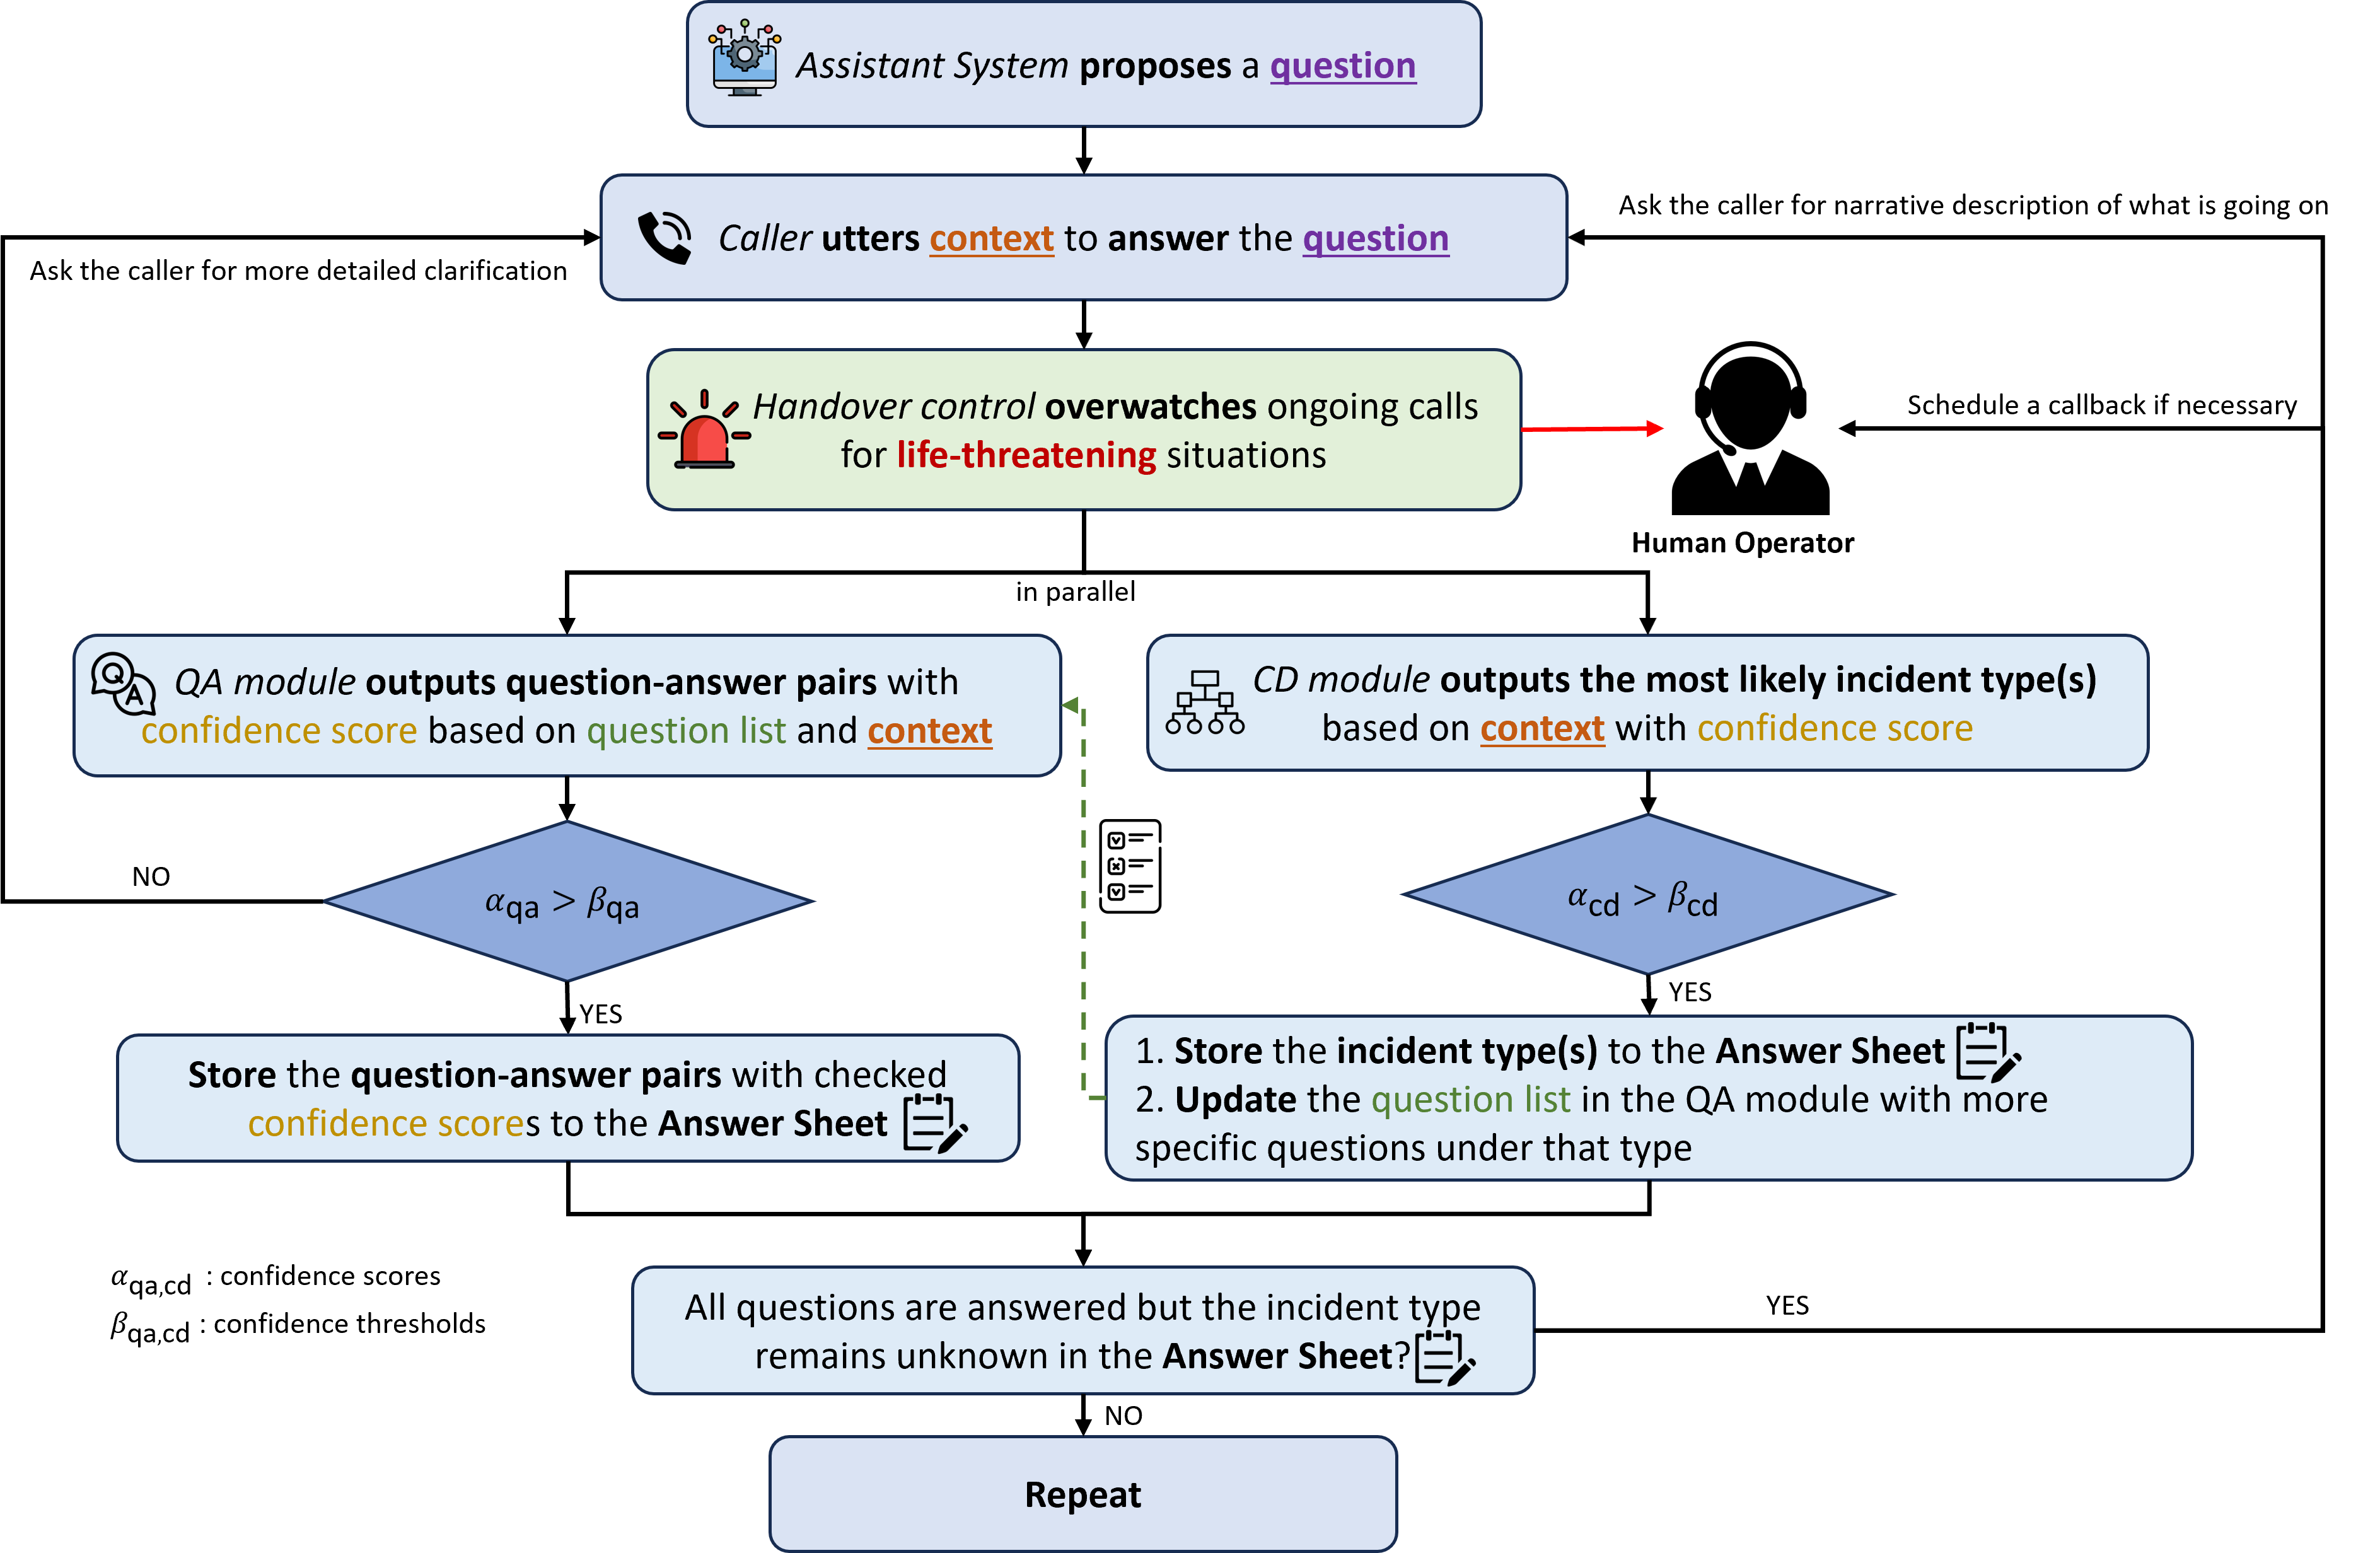
\includegraphics[width=0.9\textwidth]{figures/system_dryrun.png}
% %     \caption{Confidence-aware system choices}
% %     \label{fig:dryrun}
% %     \vspace{-0.5cm}
% % \end{figure*}


% % Confidence checking participates in both of the key modules. This module aims to not only provide the predictions to the dispatcher but also to include a \textbf{confidence score} which, by our design, indicates how the modules are confident with current outputs. A low confidence score might suggest the dispatcher carefully deciding whether to adopt the predictions.
